%! TeX program = lualatex
\documentclass[a4paper]{article} 

% packages
\usepackage{microtype}      % Slightly tweak font spacing for aesthetics
\usepackage[english]{babel} % Language hyphenation and typographical rules
\usepackage[final, colorlinks = false, urlcolor = cyan]{hyperref} 
\usepackage{changepage}     % adjust margins on the fly

\usepackage{fontspec}
\setmainfont{EB Garamond}
\setmonofont[Scale=MatchLowercase]{Deja Vu Sans Mono}

\usepackage{minted}
\usepackage{xcolor}

\usepackage{pgfplots}
\pgfplotsset{width=\textwidth,compat=1.9}

\usepackage{caption}
\newenvironment{code}{\captionsetup{type=listing}}{}
% \captionsetup[listing]{font=small, skip=0pt}
% \setlength{\abovecaptionskip}{0pt}
% \setlength{\belowcaptionskip}{5pt}

\usepackage[yyyymmdd]{datetime}
\renewcommand{\dateseparator}{--}

\usepackage{titlesec}
% \titleformat{\section}{\LARGE\bfseries}{}{}{}[\titlerule]
% \titleformat{\subsection}{\Large\bfseries}{}{0em}{}
% \titlespacing{\subsection}{0em}{-0.7em}{0em}
%
% \titleformat{\subsubsection}{\large\bfseries}{}{0em}{$\bullet$ }
% \titlespacing{\subsubsection}{1em}{-0.7em}{0em}

% margins
\addtolength{\hoffset}{-2.25cm}
\addtolength{\textwidth}{4.5cm}
\addtolength{\voffset}{-3.25cm}
\addtolength{\textheight}{5cm}
\setlength{\parskip}{0pt}
\setlength{\parindent}{0in}
% \setcounter{secnumdepth}{0}

\begin{document}
\hrule \medskip
\begin{minipage}{0.295\textwidth} 
    \raggedright
    \footnotesize 
    Name: Andrew Hayes \\
    E-mail: \href{mailto://a.hayes18@universityofgalway.ie}{\texttt{a.hayes18@universityofgalway.ie}}  \hfill\\   
    ID: 21321503 \hfill
\end{minipage}
\begin{minipage}{0.4\textwidth} 
    \centering 
    \vspace{0.4em}
    \Large 
    \textbf{CT3531} \\ 
\end{minipage}
\begin{minipage}{0.295\textwidth} 
    \raggedleft
    \today
\end{minipage}
\medskip\hrule 
\begin{center}
    \normalsize
    Assignment 02: Build \& Test OSPF Routed Network 
\end{center}
\hrule

\section{Network Topology}
\begin{figure}[H]
    \centering
    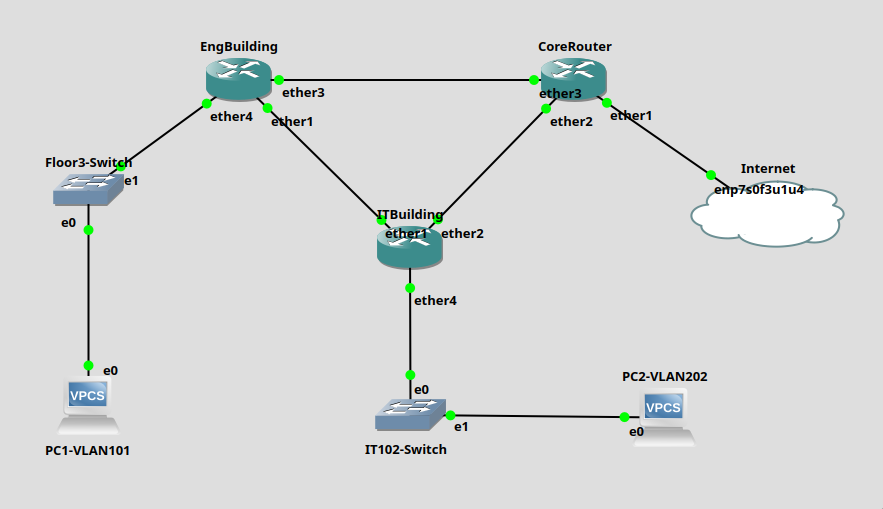
\includegraphics[width=\textwidth]{./images/topology.png}
    \caption{Network Topology}
\end{figure}

Note that the Internet device is linked to the CoreRouter device via the \verb|enp7s0f3u1u4| interface.
This is because I am running the simulation locally on my GNU/Linux laptop without any virtualisation -- \verb|enp7s0f3u1u4| is the name of the Ethernet interface on 
my laptop.
 
\section{Routers Pinging Each Other}
The following screenshots show each of the routers pinging each each router that they are directly linked to:
\begin{figure}[H]
    \centering
    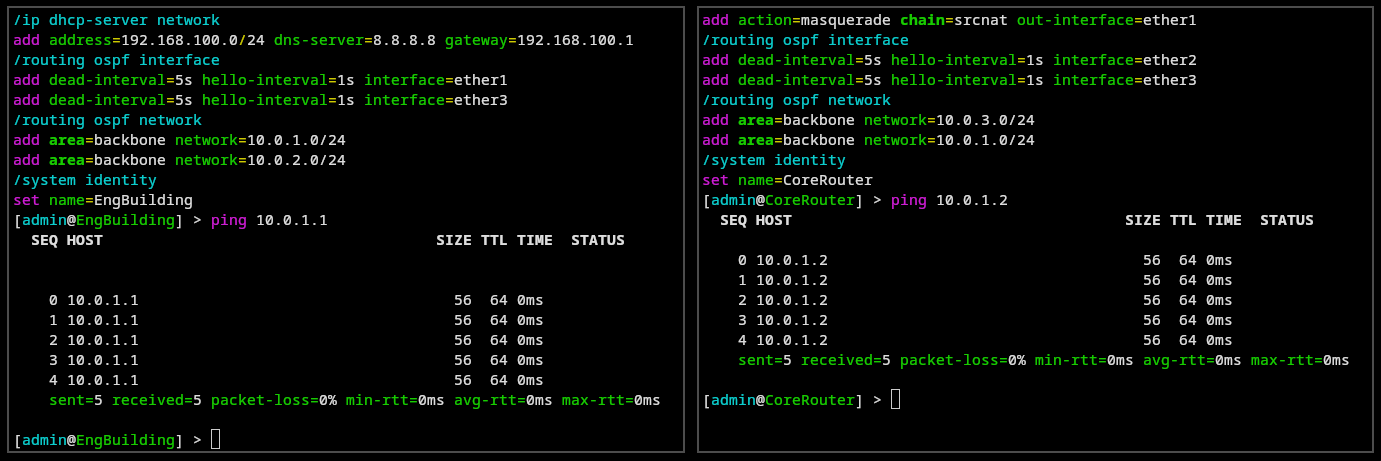
\includegraphics[width=\textwidth]{./images/eng-core.png}
    \caption{\texttt{EngBuilding} {\leftrightarrow} \texttt{CoreRouter}}
\end{figure}

\begin{figure}[H]
    \centering
    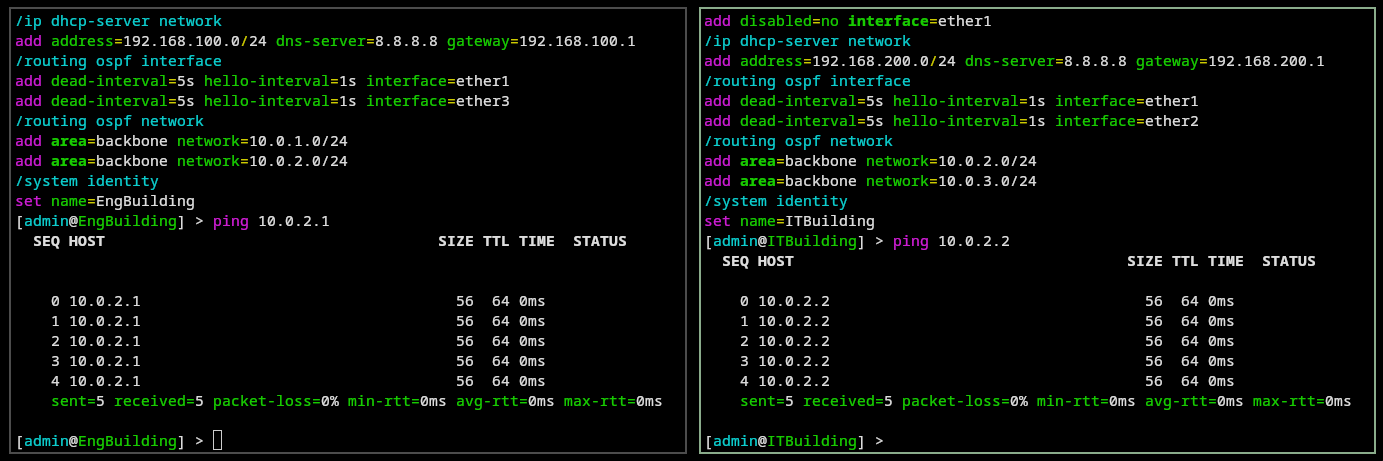
\includegraphics[width=\textwidth]{./images/eng-it.png}
    \caption{\texttt{EngBuilding} {\leftrightarrow} \texttt{ITBuilding}}
\end{figure}

\begin{figure}[H]
    \centering
    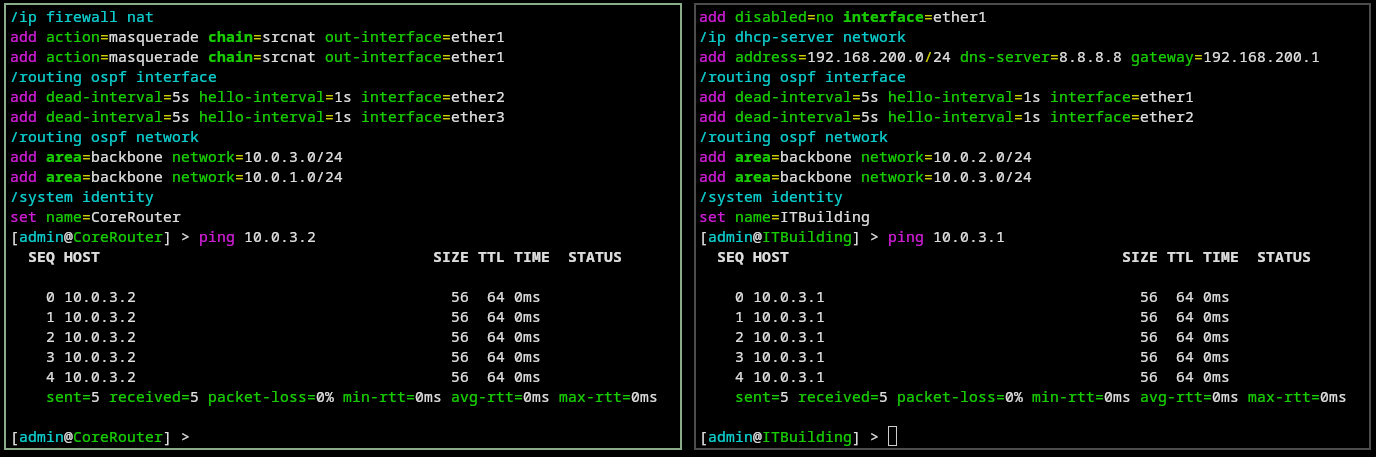
\includegraphics[width=\textwidth]{./images/core-it.png}
    \caption{\texttt{CoreRouter} {\leftrightarrow} \texttt{ITBuilding}}
\end{figure}
 
\section{Routers Pinging Each Other's Loopback Addresses}
The following screenshots show each router pinging the loopback addresses of each of the other routers:
\begin{figure}[H]
    \centering
    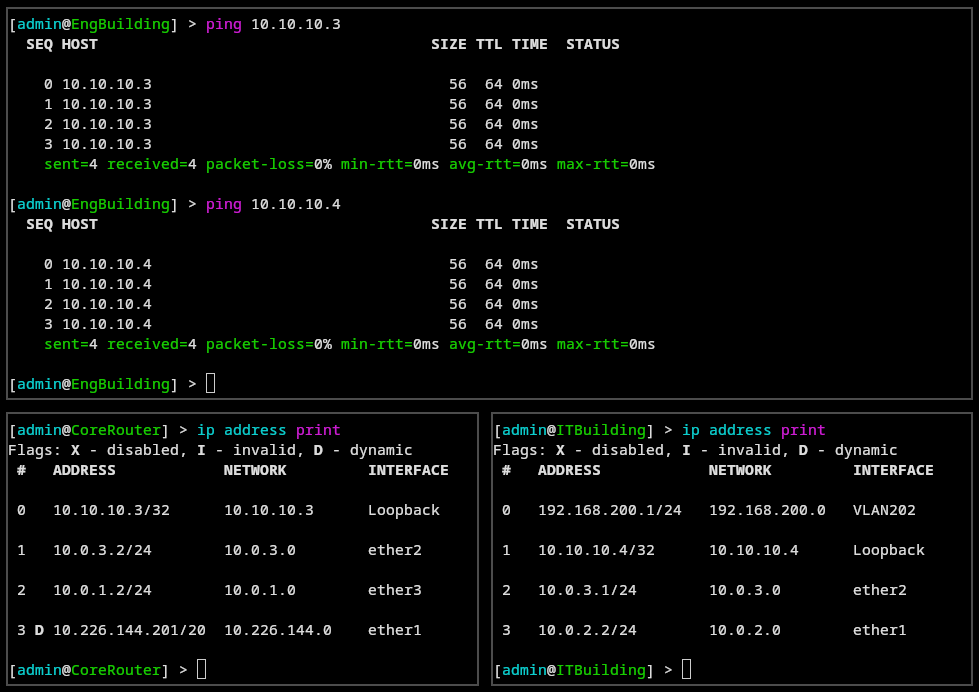
\includegraphics[width=0.8\textwidth]{./images/eng_ping_loopback.png}
    \caption{\texttt{EngBuilding} Pinging the Loopback Addresses of the Other Routers}
\end{figure}

\begin{figure}[H]
    \centering
    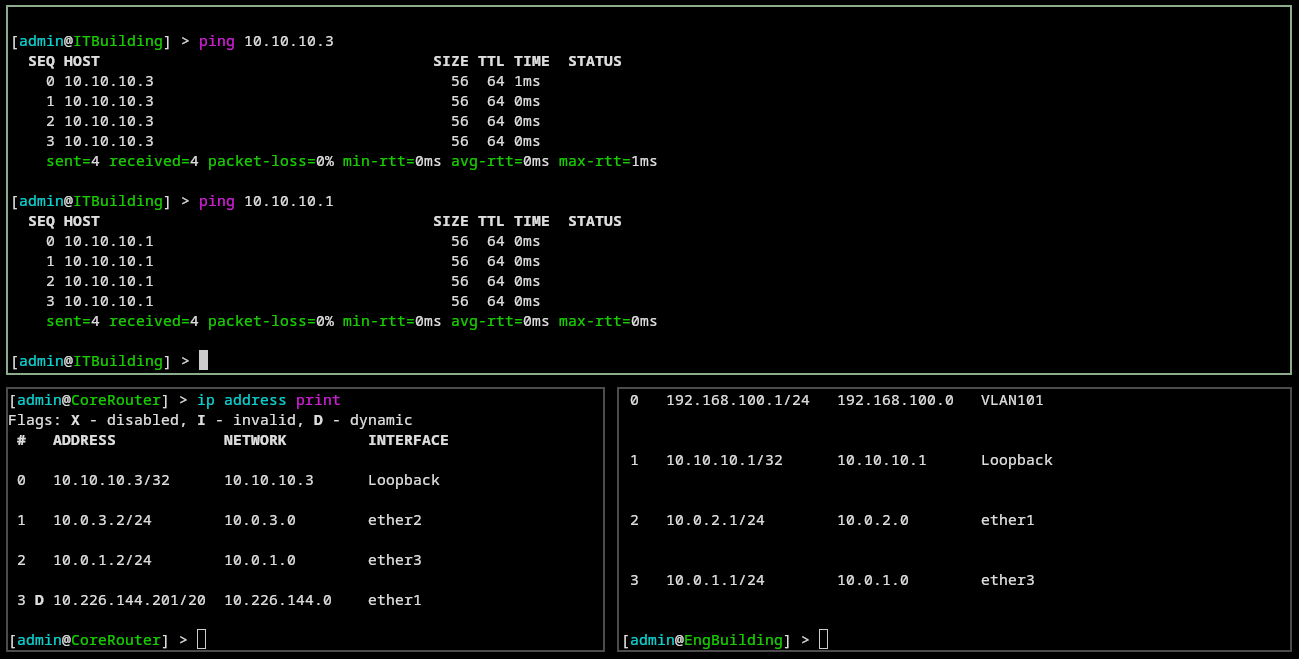
\includegraphics[width=0.8\textwidth]{./images/it_ping_loopback.png}
    \caption{\texttt{ITBuilding} Pinging the Loopback Addresses of the Other Routers}
\end{figure}

\begin{figure}[H]
    \centering
    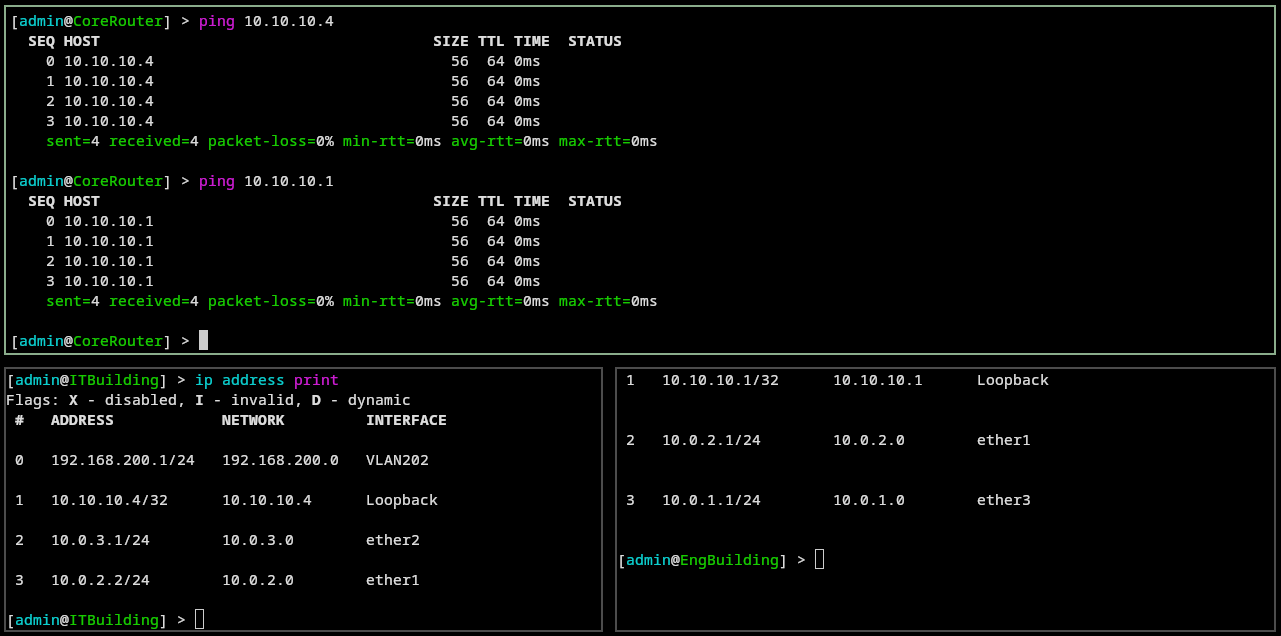
\includegraphics[width=0.8\textwidth]{./images/core_ping_loopback.png}
    \caption{\texttt{CoreRouter} Pinging the Loopback Addresses of the Other Routers}
\end{figure}

\section{VPCs Pinging Each Other}
The following screenshot shows the two PCs pinging each other:
\begin{figure}[H]
    \centering
    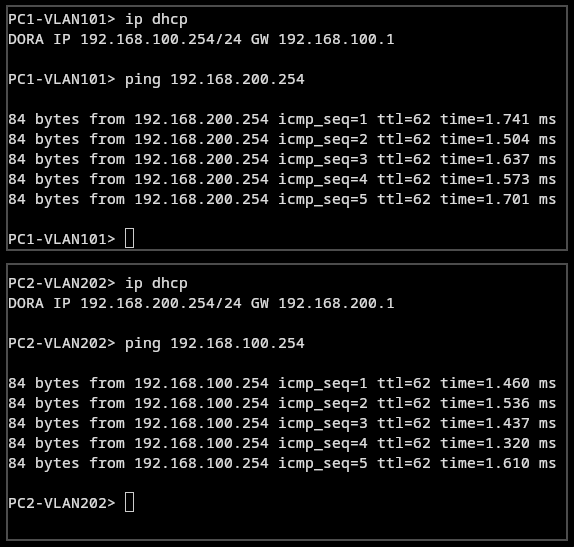
\includegraphics[width=0.45\textwidth]{./images/ping_pcs.png}
    \caption{\texttt{PC1-VLAN101} {\leftrightarrow} \texttt{PC2-VLAN202}}
\end{figure}

\section{Verify that the Internet is Reachable from All Devices}
I encountered some difficulty reaching the Internet from my devices as I was running the simulations locally on 
my GNU/Linux laptop, and my packets were getting blocked at some point by the University's firewall, both from my 
simulated devices such as the VPCs \& MikroTik routers, and when I ran a \verb|traceroute| directly from my 
laptop. 
However, the traces from my routers \& VPCs got stuck at the same IP address as the \verb|traceroute| from my real 
laptop did, which indicates to me that the Internet was reachable and operational from my network simulation, at 
least to the same extent as it was reachable from my laptop.


\begin{figure}[H]
    \centering
    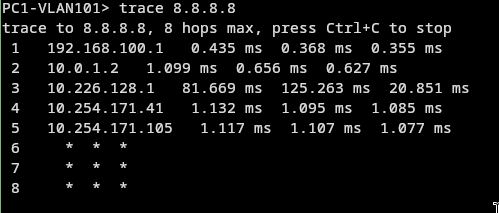
\includegraphics[width=0.6\textwidth]{./images/pc1_ping_internet.png}
    \caption{Trace to \texttt{8.8.8.8} from \texttt{PC1-VLAN101}}
\end{figure}

\begin{figure}[H]
    \centering
    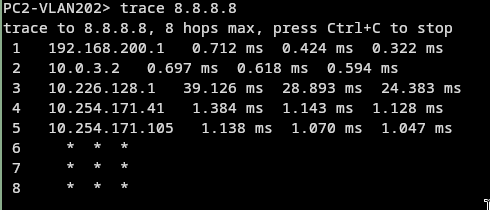
\includegraphics[width=0.6\textwidth]{./images/pc2_ping_internet.png}
    \caption{Trace to \texttt{8.8.8.8} from \texttt{PC2-VLAN202}}
\end{figure}

\begin{figure}[H]
    \centering
    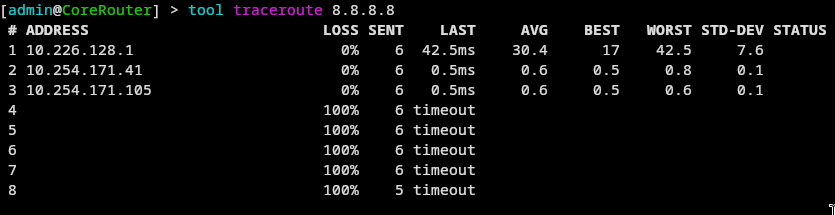
\includegraphics[width=0.8\textwidth]{./images/core_ping_internet.png}
    \caption{Trace to \texttt{8.8.8.8} from \texttt{CoreRouter}}
\end{figure}

\begin{figure}[H]
    \centering
    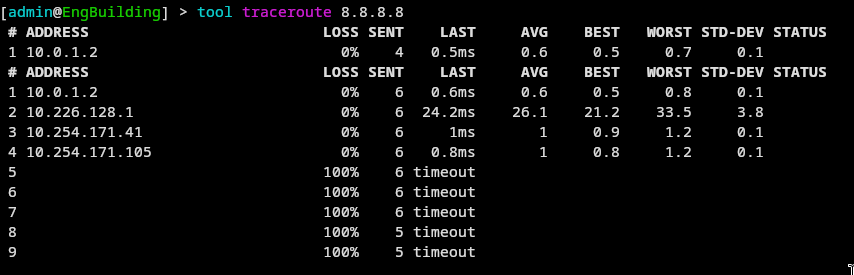
\includegraphics[width=0.8\textwidth]{./images/eng_ping_internet.png}
    \caption{Trace to \texttt{8.8.8.8} from \texttt{EngBuilding}}
\end{figure}

\begin{figure}[H]
    \centering
    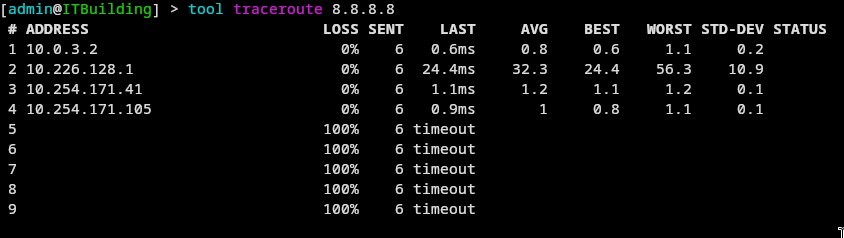
\includegraphics[width=0.8\textwidth]{./images/it_ping_internet.png}
    \caption{Trace to \texttt{8.8.8.8} from \texttt{ITBuilding}}
\end{figure}

\begin{figure}[H]
    \centering
    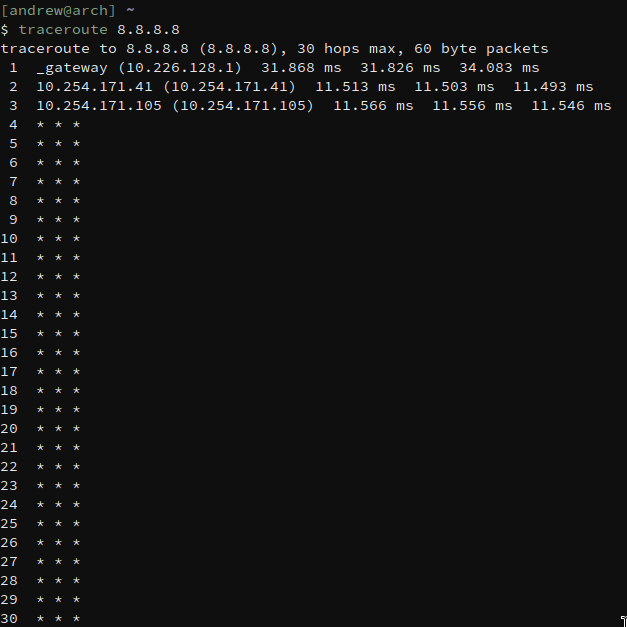
\includegraphics[width=0.7\textwidth]{./images/laptop_ping_internet.png}
    \caption{Trace to \texttt{8.8.8.8} Directly from My Laptop}
\end{figure}

\section{\texttt{CoreRouter}'s Routing Table}
\begin{figure}[H]
    \centering
    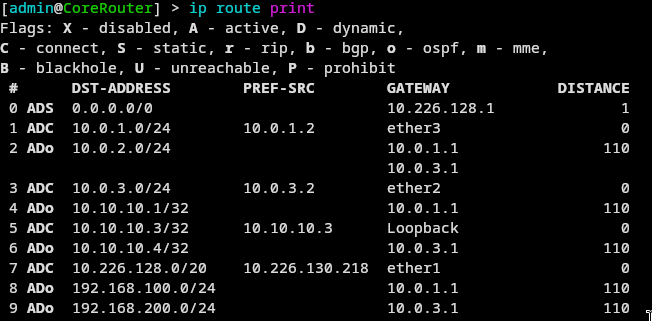
\includegraphics[width=0.7\textwidth]{./images/routing_table.png}
    \caption{\texttt{CoreRouter}'s Routing Table}
\end{figure}

Each entry in the routing table has a route number denoted \verb|#|, a flag, a destination address denoted \verb|DST-ADDRESS|, 
a preferred source denoted \verb|PREF-SRC|, a gateway denoted \verb|GATEWAY|, \& an OSPF routing distance denoted 
\verb|DISTANCE|.

The explanation of each entry is as follows:
\begin{enumerate}
\setcounter{enumi}{-1} 
    \item   This entry has a destination of \verb|0.0.0.0/0|, a gateway of \verb|10.226.144.1|, a flag of \verb|ADS| meaning 
            that it is \textbf{A}ctive, \textbf{D}ynamic (the route is dynamically learned through the routing protocol), \& 
            \textbf{S}tatic (the route is statically configured), \& a distance of 1, which means that the route is highly preferred.
            It has no preferred source.
            This entry has the destination address of \verb|0.0.0.0/0| which represents the default route -- this is where any 
            destination address that doesn't match a specific route in the routing table is sent.
            Any traffic that matches this default destination route will be forwarded to the gateway, which sends it out to
            the Internet.

    \item   This entry has a destination of \verb|10.0.1.0/24|, a preferred source of \verb|10.0.1.2|, a gateway of 
            \verb|ether3|, \& a distance of 0. 
            This destination address is that of the \verb|EngBuilding| network, and the gateway is the link from 
            \verb|CoreRouter| to \verb|EngBuilding|. 
            Its preferred source is the IP of the gateway to the \verb|EngBuilding| router on \verb|ether3|.
            Its flag is \verb|ADC| which means that it is \textbf{A}ctive, \textbf{D}ynamic, \& \textbf{C}onnected, i.e. 
            the route represents a directly connected network (that of \verb|EngBuilding|).
            It has a cost of 1, which is quite low, showing that it is highly preferred.

    \item   This entry has a destination of \verb|10.0.2.0/24|, no preferred source, a gateway of 
            \verb|10.0.1.1| or \verb|10.0.3.1|, \& a distance of 110. 
            The destination is that of the \verb|ITBuilding| network, and the two potential gateways are that of the 
            \verb|EngBuilding| router and the \verb|CoreRouter| router, indicating that the network can be reached from 
            either router.
            Its flag is \verb|ADo|, where the ``o'' represents that the route was discovered through the \textbf{O}SPF 
            protocol.
            It has a high cost of \verb|110|, which shows that it is not preferred.

    \item   This entry has a destination of \verb|10.0.3.0/24|, a preferred source of \verb|10.0.3.2|, a gateway of 
            \verb|ether2|, \& a distance of 0. 
            This is the route to the \verb|ITBuilding| network and its preferred source is from within that network.
            Its flag is \verb|ADC| meaning that it is active, dynamic, \& connected and the distance of 0 indicates it is 
            highly preferred, likely because it is directly connected to the router.

    \item   This entry has a destination of \verb|10.10.10.1/32|, no preferred source, a gateway of 
            \verb|10.0.1.1|, \& a distance of 110. 
            The destination is the loopback address of the \verb|EngBuilding| router and the gateway is that of the link 
            that joins \verb|EngBuilding| \& \verb|CoreRouter|.
            Its flag is \verb|ADo| indicating that it was discovered via the OSPF protoocl and the distance of 110
            indicates that it is not preferred.

    \item   This entry has a destination of \verb|10.10.10.3/32|, a preferred source of \verb|10.10.10.3|, a gateway of 
            \verb|Loopback|, \& a distance of 0. 
            The destination is the loopback address of the \verb|CoreRouter| and the gateway is also the loopback address.
            Its flag is \verb|ADo| indicating that it was discovered via the OSPF protoocl and the distance of 0
            indicates that it is highly preferred, likely because it is literally the same device.

    \item   This entry has a destination of \verb|10.10.10.4/32|, no preferred source, a gateway of 
            \verb|10.0.3.1|, \& a distance of 110. 
            The destination is the loopback address of the \verb|ITBuilding| router and the gateway is that of the link 
            that joins \verb|ITBuilding| \& \verb|CoreRouter|.
            Its flag is \verb|ADo| indicating that it was discovered via the OSPF protoocl and the distance of 110
            indicates that it is not preferred.

    \item   This entry has a destination of \verb|10.226.128.0/32|, a preferred source of \verb|10.226.130.218|, a
            gateway of \verb|ether1|, \& a distance of 0. 
            The destination address is the same IP as the gateway of route \verb|0|, as this is the address out onto the 
            internet, via a University router.
            Its flag is \verb|ADC| indicating that it is directly connected to \verb|CoreRouter| and the distance of 0
            indicates that it is highly preferred, likely because it is directly connected.

    \item   This entry has a destination of \verb|192.168.100.0/24|, no preferred source, a
            gateway of \verb|10.0.1.1|, \& a distance of 110. 
            The destination address is that of \verb|VLAN101|, and its gateway is the address of the link between 
            \verb|CoreRouter| \& \verb|EngBuilding|, as \verb|VLAN101| is only accessible through \verb|EngBuilding|.
            Its flag is \verb|ADo| indicating that it was discovered via the OSPF protocol and the distance of 110
            indicates that it is not preferred.

    \item   This entry has a destination of \verb|192.168.200.0/24|, no preferred source, a
            gateway of \verb|10.0.3.1|, \& a distance of 110. 
            The destination address is the IP of \verb|VLAN202|, and its gateway is the address of the link between 
            \verb|CoreRouter| \& \verb|ITBuilding|, as \verb|VLAN202| is only accessible through \verb|ITBuilding|.
            Its flag is \verb|ADo| indicating that it was discovered via the OSPF protocol and the distance of 110
            indicates that it is not preferred.
\end{enumerate}

\section{What if Each Router Wasn't Set Up to Redistribute Connected Networks?}
If each router was not set up to redistribute connected networks, the other routers would not be aware of the networks 
that were directly connected to the other routers, and therefore \verb|ITBuilding| \& \verb|CoreRouter| would not be aware 
of the existence of \verb|VLAN101|, and \verb|EngBuilding| \& \verb|CoreRouter| would not be aware of the existence of 
\verb|VLAN202|.
This would mean that these networks would not be included in the routing tables of the routers that are not directly 
connected to them and therefore they would not be reachable from these routers using OSPF routing.
This would prevent the VPCs from being able to ping each other: if \verb|PC1-VLAN101| tried to ping \verb|PC2-VLAN202|, 
\verb|EngBuilding| would not know where to route the traffic next, as \verb|ITBuilding| wouldn't have told \verb|EngBuilding| 
that it was connected to \verb|VLAN202|.
The inverse would also be true if \verb|PC2-VLAN202| tried to ping \verb|PC1-VLAN101|.

\section{Traceroute from \texttt{PC1-VLAN101} to \texttt{PC2-VLAN202}}
\begin{figure}[H]
    \centering
    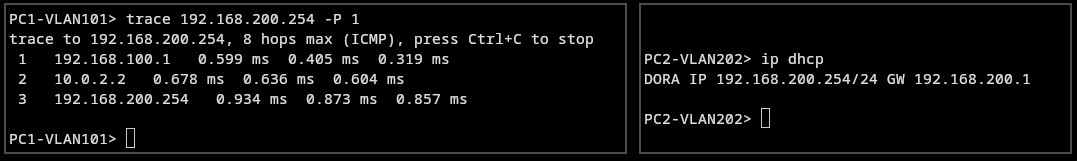
\includegraphics[width=\textwidth]{./images/trace_pcs.png}
    \caption{Trace from \texttt{PC1-VLAN101} to \texttt{PC2-VLAN202}}
\end{figure}

\subsection{Explanation of the Route Taken}
The trace from \verb|PC1-VLAN101| to \verb|PC2-VLAN202| takes three hops:
\begin{enumerate}
    \item   \verb|192.168.100.1|: the gateway to \verb|VLAN101| on the \verb|EngBuilding| router.
            Any traffic entering or exiting \verb|VLAN101| must pass through this gateway.

    \item   \verb|10.0.2.2|: the gateway to the \verb|ITBuilding| router on its \verb|ether1| interface, which links 
            \verb|EngBuilding| to \verb|ITBuilding|.

    \item   \verb|192.168.200.254|: the VPC \verb|PC2-VLAN202| itself, which is naturally the final destination in a 
            successful trace to this device.
\end{enumerate}

\section{Long Ping from \texttt{PC1-VLAN101} to \texttt{PC2-VLAN202}}
Below is the output of a 30 seconds-long ping that was made from \verb|PC1-VLAN101| to \verb|PC2-VLAN202|. 
While this ping was running, the link from the \verb|EngBuilding| router to the \verb|ITBuilding| router was suspended.
\begin{figure}[H]
    \centering
    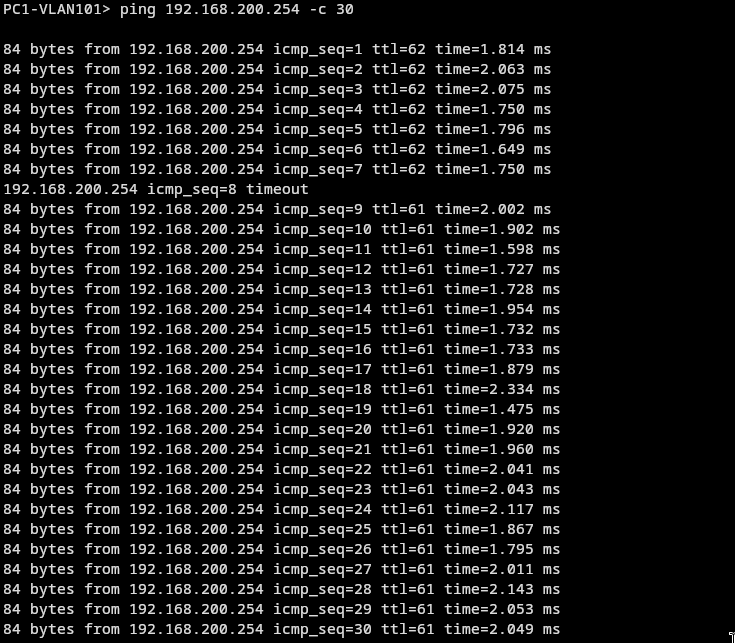
\includegraphics[width=0.8\textwidth]{./images/long_ping.png}
    \caption{Long Ping from \texttt{PC1-VLAN101} to \texttt{PC2-VLAN202}}
\end{figure}

The \verb|EngBuilding| {\leftrightarrow} \verb|ITBuilding| link was suspended just before the 8\textsuperscript{th} packet 
was sent, resulting in this packet being dropped as it was sent along a route that no longer existed. 
OSPF kicked in very quickly and the traffic was re-routed after just one lost packet. 
It is quite obvious from looking at the network topology that the only other way the traffic could have been routed was 
from \verb|EngBuilding| {\rightarrow} \verb|CoreRouter| {\rightarrow} \verb|ITBuilding|, which requires an extra hop. 
This path, being longer \& not direct, would have not been preferred by OSPF when there was a link between \verb|EngBuilding| 
\& \verb|ITBuilding|, but now that it's the best possible option, it will make use of it.
We can see why this route was not preferred by the OSPF protocol, as it usually takes noticeably longer than the original route.

\begin{figure}[H]
    \centering
    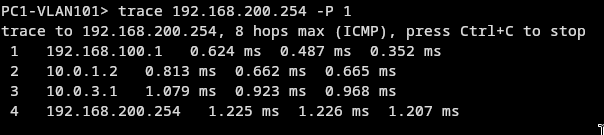
\includegraphics[width=0.8\textwidth]{./images/redo_trace.png}
    \caption{Trace from \texttt{PC1-VLAN101} to \texttt{PC2-VLAN202} After Suspending the \texttt{EngBuilding} {\leftrightarrow} \texttt{ITBuilding} Link}
\end{figure}

Comparing the above trace to the one ran previously, we can see that there is one extra hop now that the 
\verb|EngBuilding| {\leftrightarrow} \verb|ITBuilding| link has been suspended and that it does not go through the 
\verb|10.0.2.2| gateway it did when we first ran the ping.
That gateway was the one between \verb|EngBuilding| \& \verb|ITBuilding|, which is of course now gone. 
Instead, the traffic travels over the link between \verb|EngBuilding| \& \verb|CoreRouter| (\verb|10.0.1.2|) and then over 
the link between \verb|CoreRouter| \& \verb|ITBuilding| (\verb|10.0.3.1|), as expected.

\section{Packet Capture on Link from \texttt{EngBuilding} to \texttt{CoreRouter}}
I ran a packet capture on the link from \texttt{EngBuilding} to \texttt{CoreRouter} and restored the link from 
\verb|EngBuilding| to \verb|CoreRouter|, then stopped the packet capture after around 30 seconds to ensure that OSPF had 
detected the topology changed and re-converged.
Nine LSA packets were captured:
\begin{enumerate}
    \item   The first two packets are LS Update packets originating from \verb|EngBuilding| \& \verb|ITBuilding|.
    The first originated from \verb|10.0.1.2| advertising \verb|10.10.10.4| (\verb|ITBuilding|) while the second originated 
    from \verb|10.0.10.1| advertising \verb|10.10.10.1| (\verb|EngBuilding|).
    This is the routers announcing that they can be reached over this new topology.

    \item   The next two packets are LS Acknowledgements, originating from the same two routers, each acknowledging the 
            other router's update.

    \item   The next packet is an LS Update originating from \verb|10.0.1.1| advertising \verb|10.10.10.1| (\verb|EngBuilding|)
            again.
            Another packet from the same origin then advertised \verb|10.10.10.4| (\verb|ITBuilding|).
            This being the IP address which originally advertised \verb|EngBuilding| shows that it has learnt that \verb|ITBuilding| 
            is reachable to it from its advertisement.
            \verb|10.0.1.2| then sent a packet advertising \verb|ITBuilding| again.

    \item   \verb|10.0.1.1| acknowledged \verb|10.0.1.2|'s advertisement of \verb|10.10.10.4|, and \verb|10.0.1.2| 
            acknowledged \verb|10.0.1.1|'s advertisement of \verb|EngBuilding|.
\end{enumerate}

\begin{figure}[H]
    \centering
    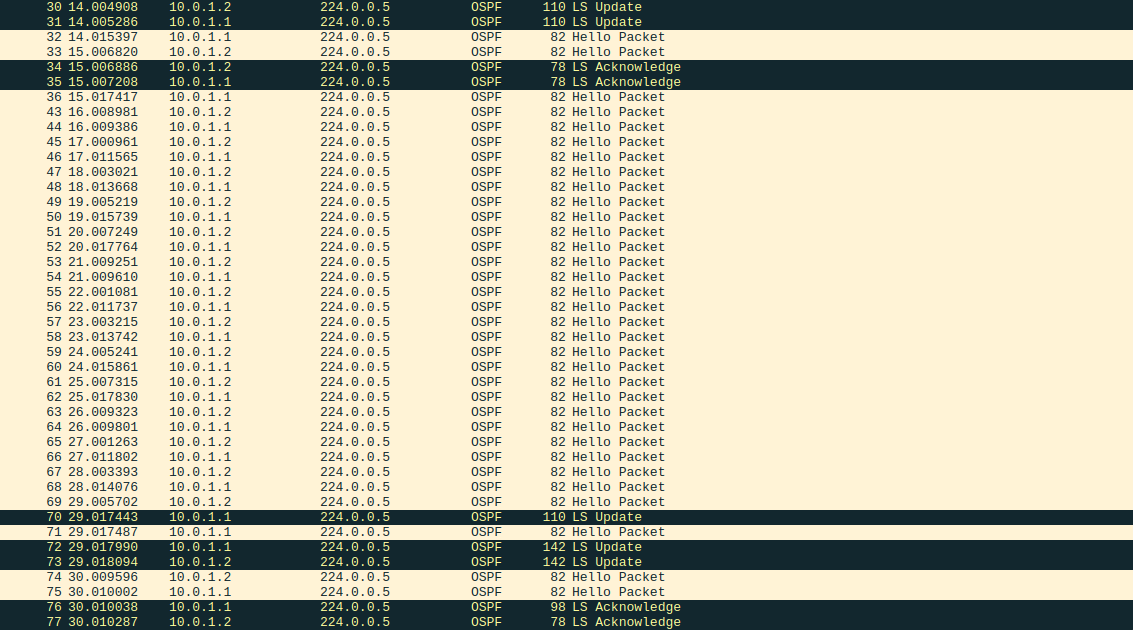
\includegraphics[width=\textwidth]{./images/pcap.png}
    \caption{OSPF Packets Captured on the \texttt{EngBuilding} {\leftrightarrow} \texttt{CoreRouter} Link}
\end{figure}


\end{document}
